\chapter{Logikgatter}
\section{Wahrheitswerttabelle}

\begin{table}[H]
    \centering
    \def\arraystretch{1.3}
    \rowcolors{2}{gray!15}{white}
    \begin{tabular}{|c|c!{\vrule width 1.5pt}c|c|c!{\vrule width 1.5pt}c|c|c|c|}
        \rowcolor{gray!50}
        \hline
        Zähler & Würfel & $z_2$ & $z_1$ & $z_0$ & $w_3$ & $w_2$ & $w_1$ & $w_0$ \\
        \hline
        0      & 1      & 0     & 0     & 0     & 1     & 1     & 1     & 0     \\
        \hline
        1      & 2      & 0     & 0     & 1     & 1     & 1     & 0     & 1     \\
        \hline
        2      & 3      & 0     & 1     & 0     & 1     & 1     & 0     & 0     \\
        \hline
        3      & 4      & 0     & 1     & 1     & 1     & 0     & 0     & 1     \\
        \hline
        4      & 5      & 1     & 0     & 0     & 1     & 0     & 0     & 0     \\
        \hline
        5      & 6      & 1     & 0     & 1     & 0     & 0     & 0     & 1     \\
        \hline
    \end{tabular}
    \caption{Mapping: Zähler auf Würfel}
    \label{tab:sample}
\end{table}

\section{KV-Diagramme und vereinfachte Formeln}

\begin{table}[H]
    \centering
    \renewcommand{\arraystretch}{7.5}
    \begin{tabular}{c@{\hskip 1.5cm}c}
        \begin{tikzpicture}
            \matrix[matrix of nodes, nodes={draw, minimum size=1cm, anchor=center, text height=1.5ex, text depth=.25ex}] (kmap) {
            |[]| 1 & |[]| 1 & |[]| 1 & |[]| 1 \\
            |[]| 1 & |[]| 0 & |[]| x & |[]| x \\
            };

            % Add decimal numbers in the bottom right corner of each cell
            \foreach \i/\j/\num in {1/1/0, 1/2/1, 1/3/3, 1/4/2, 2/1/4, 2/2/5, 2/3/7, 2/4/6} {
                    \node[anchor=south east, font=\tiny] at (kmap-\i-\j.south east) {\num};
                }

            % Add variable names for columns
            \node[above=0.2cm of kmap-1-1.north] {$\overline{z}_0$};
            \node[above=0.2cm of kmap-1-2.north] {$z_0$};
            \node[above=0.2cm of kmap-1-3.north] {$z_0$};
            \node[above=0.2cm of kmap-1-4.north] {$\overline{z}_0$};

            % Add variable names for columns on the bottom
            \node[below=0.2cm of kmap-2-1.south] {$\overline{z}_1$};
            \node[below=0.2cm of kmap-2-2.south] {$\overline{z}_1$};
            \node[below=0.3cm of kmap-2-3.south] {$z_1$};
            \node[below=0.3cm of kmap-2-4.south] {$z_1$};

            % Add variable names for rows on the right
            \node[right=0.2cm of kmap-1-4.east] {$\overline{z}_2$};
            \node[right=0.2cm of kmap-2-4.east] {$z_2$};

            % Mark areas to simplify with multiple semi-transparent backgrounds
            \draw[fill=yellow, fill opacity=0.3, draw=none] (kmap-1-1.north west) rectangle (kmap-1-4.south east);

            \draw[fill=blue, fill opacity=0.3, draw=none] (kmap-1-1.north west) rectangle (kmap-2-1.south east);

            \draw[fill=blue, fill opacity=0.3, draw=none] (kmap-1-4.north west) rectangle (kmap-2-4.south east);

            \node[below=1cm of kmap] {$w_3 = \overline{z}_2 \ \lor \ \overline{z}_0$};
        \end{tikzpicture} &
        \begin{tikzpicture}
            \matrix[matrix of nodes, nodes={draw, minimum size=1cm, anchor=center, text height=1.5ex, text depth=.25ex}] (kmap) {
            |[]| 1 & |[]| 1 & |[]| 0 & |[]| 1 \\
            |[]| 0 & |[]| 0 & |[]| x & |[]| x \\
            };

            % Add decimal numbers in the bottom right corner of each cell
            \foreach \i/\j/\num in {1/1/0, 1/2/1, 1/3/3, 1/4/2, 2/1/4, 2/2/5, 2/3/7, 2/4/6} {
                    \node[anchor=south east, font=\tiny] at (kmap-\i-\j.south east) {\num};
                }

            % Add variable names for columns
            \node[above=0.2cm of kmap-1-1.north] {$\overline{z}_0$};
            \node[above=0.2cm of kmap-1-2.north] {$z_0$};
            \node[above=0.2cm of kmap-1-3.north] {$z_0$};
            \node[above=0.2cm of kmap-1-4.north] {$\overline{z}_0$};

            % Add variable names for columns on the bottom
            \node[below=0.2cm of kmap-2-1.south] {$\overline{z}_1$};
            \node[below=0.2cm of kmap-2-2.south] {$\overline{z}_1$};
            \node[below=0.3cm of kmap-2-3.south] {$z_1$};
            \node[below=0.3cm of kmap-2-4.south] {$z_1$};

            % Add variable names for rows on the right
            \node[right=0.2cm of kmap-1-4.east] {$\overline{z}_2$};
            \node[right=0.2cm of kmap-2-4.east] {$z_2$};

            % Mark areas to simplify with multiple semi-transparent backgrounds
            \draw[fill=yellow, fill opacity=0.3, draw=none] (kmap-1-1.north west) rectangle (kmap-1-2.south east);

            \draw[fill=blue, fill opacity=0.3, draw=none] (kmap-1-4.north west) rectangle (kmap-2-4.south east);

            \node[below=1cm of kmap] {$w_2 = \overline{z}_2 \overline{z}_1 \ \lor \ z_1 \overline{z}_0$};
        \end{tikzpicture}

        \\

        \begin{tikzpicture}
            \matrix[matrix of nodes, nodes={draw, minimum size=1cm, anchor=center, text height=1.5ex, text depth=.25ex}] (kmap) {
            |[]| 1 & |[]| 0 & |[]| 0 & |[]| 0 \\
            |[]| 0 & |[]| 0 & |[]| x & |[]| x \\
            };

            % Add decimal numbers in the bottom right corner of each cell
            \foreach \i/\j/\num in {1/1/0, 1/2/1, 1/3/3, 1/4/2, 2/1/4, 2/2/5, 2/3/7, 2/4/6} {
                    \node[anchor=south east, font=\tiny] at (kmap-\i-\j.south east) {\num};
                }

            % Add variable names for columns
            \node[above=0.2cm of kmap-1-1.north] {$\overline{z}_0$};
            \node[above=0.2cm of kmap-1-2.north] {$z_0$};
            \node[above=0.2cm of kmap-1-3.north] {$z_0$};
            \node[above=0.2cm of kmap-1-4.north] {$\overline{z}_0$};

            % Add variable names for columns on the bottom
            \node[below=0.2cm of kmap-2-1.south] {$\overline{z}_1$};
            \node[below=0.2cm of kmap-2-2.south] {$\overline{z}_1$};
            \node[below=0.3cm of kmap-2-3.south] {$z_1$};
            \node[below=0.3cm of kmap-2-4.south] {$z_1$};

            % Add variable names for rows on the right
            \node[right=0.2cm of kmap-1-4.east] {$\overline{z}_2$};
            \node[right=0.2cm of kmap-2-4.east] {$z_2$};

            % Mark areas to simplify with multiple semi-transparent backgrounds
            \draw[fill=yellow, fill opacity=0.3, draw=none] (kmap-1-1.north west) rectangle (kmap-1-1.south east);

            \node[below=1cm of kmap] {$w_1 = \overline{z}_2 \overline{z}_1 \overline{z}_0$};
        \end{tikzpicture} &
        \begin{tikzpicture}
            \matrix[matrix of nodes, nodes={draw, minimum size=1cm, anchor=center, text height=1.5ex, text depth=.25ex}] (kmap) {
            |[]| 0 & |[]| 1 & |[]| 1 & |[]| 0 \\
            |[]| 0 & |[]| 1 & |[]| x & |[]| x \\
            };

            % Add decimal numbers in the bottom right corner of each cell
            \foreach \i/\j/\num in {1/1/0, 1/2/1, 1/3/3, 1/4/2, 2/1/4, 2/2/5, 2/3/7, 2/4/6} {
                    \node[anchor=south east, font=\tiny] at (kmap-\i-\j.south east) {\num};
                }

            % Add variable names for columns
            \node[above=0.2cm of kmap-1-1.north] {$\overline{z}_0$};
            \node[above=0.2cm of kmap-1-2.north] {$z_0$};
            \node[above=0.2cm of kmap-1-3.north] {$z_0$};
            \node[above=0.2cm of kmap-1-4.north] {$\overline{z}_0$};

            % Add variable names for columns on the bottom
            \node[below=0.2cm of kmap-2-1.south] {$\overline{z}_1$};
            \node[below=0.2cm of kmap-2-2.south] {$\overline{z}_1$};
            \node[below=0.3cm of kmap-2-3.south] {$z_1$};
            \node[below=0.3cm of kmap-2-4.south] {$z_1$};

            % Add variable names for rows on the right
            \node[right=0.2cm of kmap-1-4.east] {$\overline{z}_2$};
            \node[right=0.2cm of kmap-2-4.east] {$z_2$};

            % Mark areas to simplify with multiple semi-transparent backgrounds
            \draw[fill=yellow, fill opacity=0.3, draw=none] (kmap-1-2.north west) rectangle (kmap-2-3.south east);

            \node[below=1cm of kmap] {$w_0 = z_0$};
        \end{tikzpicture}
    \end{tabular}
    \label{tab:logic_gates}
\end{table}

\section{Aufbau}
\begin{figure}[H]
    \centering
    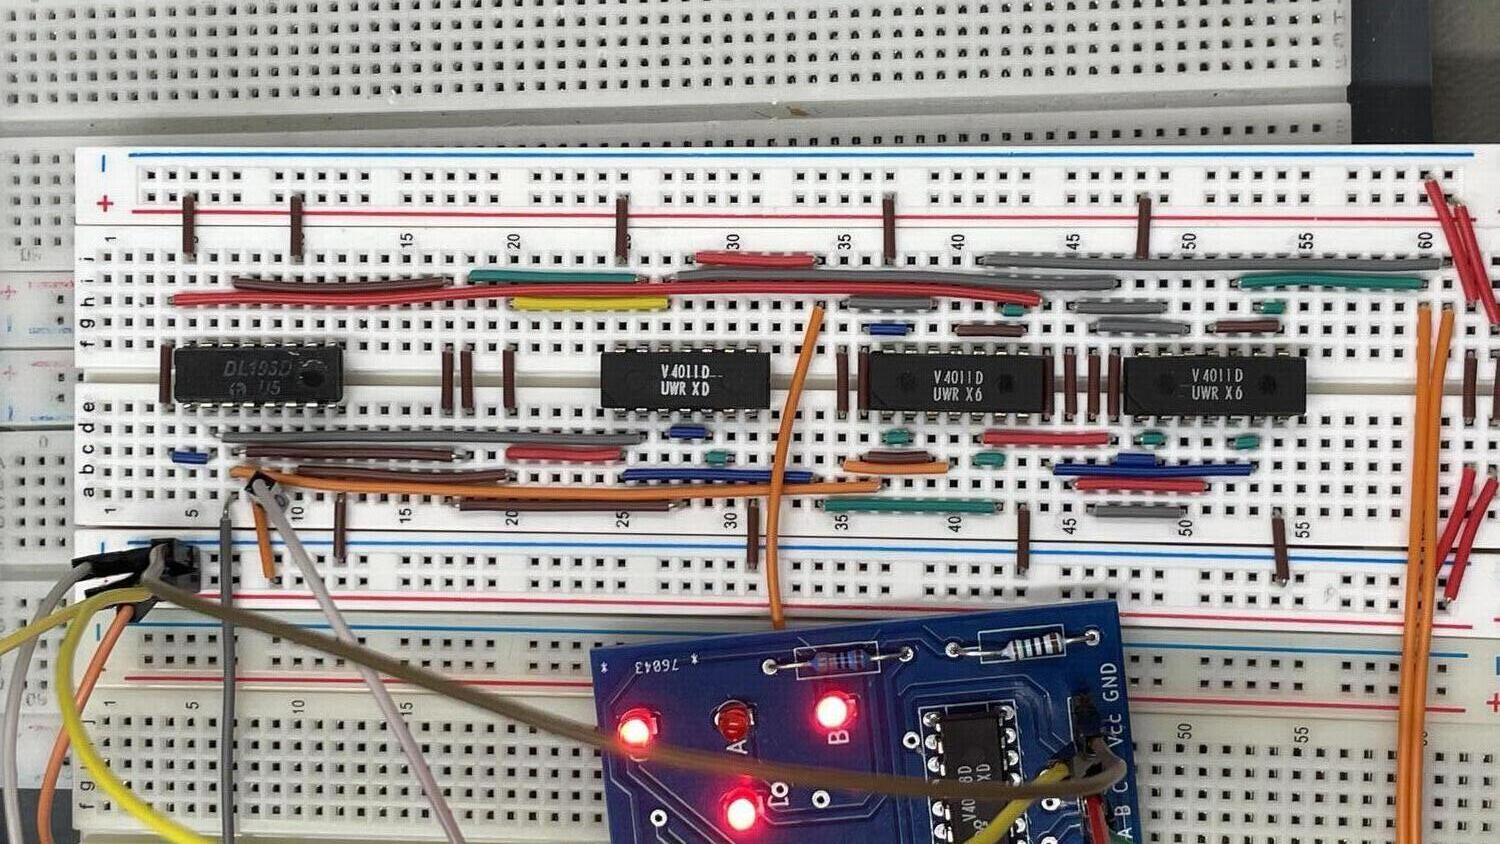
\includegraphics[width=0.8\textwidth]{dice_nand.jpeg}
    \caption{Aufbau der Schaltung mit 3 NAND-Gattern}
    \label{fig:aufbau}
\end{figure}